\chapter{Vorgehen}
- was für frameworks wurden verwendet (vs code, react, xstate, chakra ui)



\begin{figure}[h]
    \centering
    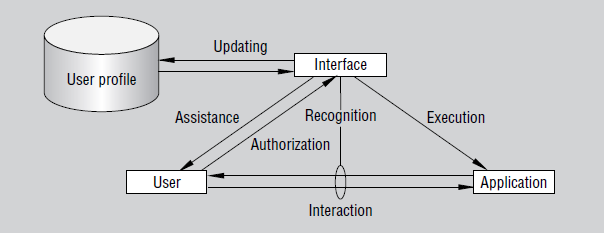
\includegraphics[height=.385\textwidth]{Shematic-AUI.png}
    \caption{Schematic of an adaptive User Interface}
\end{figure}
\newpage
The interface tracks interaction between a user and an application software system and tries to identify consistent user behavior patterns.
On the basis of these patterns, it can interact with the software on the user’s behalf whenever the user authorizes the interface to do
so. The interface might take a while to detect user patterns if it starts from scratch every time the user uses the software. Alternatively,
the AUI can build a user profile that includes all the patterns recognized in past interaction sessions. As it detects new patterns, it updates
the profile.

\chapter{Umsetzung}

